\documentclass[11pt,a4paper]{article}

\usepackage{graphicx}
\usepackage{amsthm}

\theoremstyle{definition}
\newtheorem{definition}{Definizione}[section]


\begin{document}
\title{Reti di Calcolatori a.a. 2019/2020}
\author{Francesco Iannelli}
\date{September 16, 2019}
\maketitle

\newpage

\tableofcontents
\newpage

\section{Introduzione al corso}
email: federica.paganelli@unipi.it\newline
modalità d'esame: prova scritta (compitini) e orale (facoltativo) più\newline
laboratorio che prevede progetto e orale. \newline
\underline{\textbf{N.B. Si accede alla prova orale di laboratorio solo dopo aver passato lo scritto.}}

\section{Cenni di modelli stratificati}
Sono architetture di comunicazione a strati. \newline
Concetti generali:
\begin{itemize}
	\item Stratificazione
	\item Information hiding
	\item Separation of concerns
\end{itemize}
Due modelli: \textbf{ISO/OSI} (approccio top-down) e \textbf{Stack TCP/IP} (approccio bottom-up), quest ultimo vincente.\newline
Idea chiave: \underline{suddivisone in sottoproblemi.}
\begin{figure}[!h]
	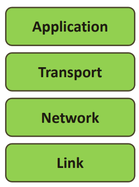
\includegraphics{Immagini/Modelli_Strat.png}
	\centering
	\caption{Modello stratificato}
\end{figure}

\pagebreak

\subsection{Livello applicativo}
Fanno parte del livello applicativo:
\begin{itemize}
	\item Identificativi delle risorse: URL, URI e URN.
	\item Il web: user agents, protocollo http.
	\item Protocollo FTP.
	\item TELNET: servizio di terminale virtuale.
	\item Posta elettronica.
	\item Sistema dei nomi DNS a dominio e la risoluzione dei nomi: iterativa e ricorsiva.
	\item molto altro ancora...
\end{itemize}

\subsection{Livello di trasporto}
Due tecnologie degne di nota:
\begin{enumerate}
	\item Protocollo \textbf{TCP}: \textbf{connection-oriented}, \textit{orientato alla connessione}.
	\item Protocollo \textbf{UDP}: \textbf{connection-less}, molto più leggero, prende dati applicativi e li affida allo strato IP, \underline{NON} da garanzie di consegna nè di ordine.
\end{enumerate}

\subsection{Livello rete}
Nel livello rete si ricava un percorso dall'host sorgente all'host destinatario usando le informazioni che si trovano nell'IP.\newline
Verrà trattato il protocollo Ipv4 e introdotto il protocollo Ipv6.

\subsection{Livello link}
Si occupa di gestire il collegamento tra due nodi \textbf{adiacenti}.
La tecnologia principale è l'\textbf{ethernet}.
\pagebreak

\section{Introduzione alle reti}
\textit{Cos'è una rete? Quante tipologie di reti ci sono? Cos'è internet?}

\theoremstyle{definition}
\begin{definition}
	Una \textbf{rete} è un'interconnessione di dispositivi in grado di scambiarsi e interpretare le informazioni. Comprende sistemi terminali e intermedi: \textit{e.g. router, switch e modem.}
\end{definition}
I sistemi terminali si possono dividere in due tipi: \textbf{host} e \textbf{server}, sull'host girano le applicazioni utente mentre il server esegue programmi che forniscono servizi applicativi ad applicazioni. \newline \textit{N.B. il termine host può essere usato per indicare anche un server. \newline L'host, infatti, può essere sia un server sia il terminale di un utente che esegue un'applicazione client, più generalmente \textbf{l'host è una macchina}.}

\theoremstyle{definition}
\begin{definition}
	Una rete è formata da \textbf{dispositivi} e da \textbf{tecnologie}.
\end{definition}

\subsection{LAN}
Acronimo di \textbf{L}ocal \textbf{A}rea \textbf{N}etwork, è
una rete di area geografica limitata collegata attraverso una tecnologia ethernet \textbf{bus} o ethernet \textbf{switch}:
\begin{figure}[!h]
	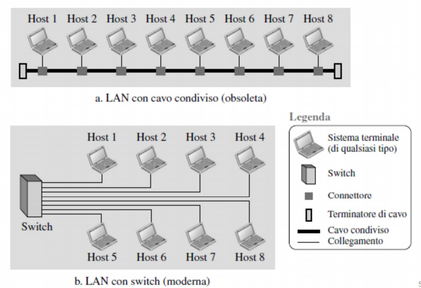
\includegraphics[width=\textwidth]{Immagini/LAN.png}
	\centering
\end{figure}

\newpage

Ciascun host ha un cavo che lo collega allo switch e a ogni porta dello switch corrisponde un host. Lo \textbf{switch} possiede una tecnologia di autoapprendimento ed è una componente del \textbf{livello link}.

\subsection{WAN}
Acronimo di \textbf{W}ide \textbf{A}rea \textbf{N}etwork, è una rete di area geografica estesa: è composta da due o più reti collegate tramite un mezzo di trasmissione. Le reti coinvolte potrebbero anche essere reti LAN. \textit{(e il link potrebbe essere affittato a un'azienda da un operatore di telefonia).}
\begin{figure}[!h]
	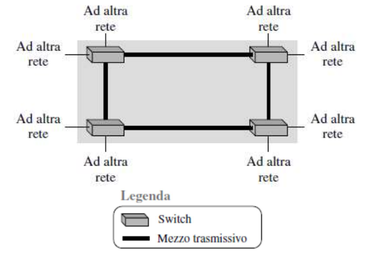
\includegraphics[width=\textwidth]{Immagini/WAN_Switch.png}
	\centering
	\caption{Un esempio di WAN a cavo condiviso e a commutazione.\newline
		Le WAN permettono l'esistenza di \textbf{percorsi alternativi} e la \textbf{divisione del traffico}.}
\end{figure}

\newpage

\subsection{Internetwork}
L'internetwork è un sistema in cui ci sono più reti composte, capaci di scambiarsi informazioni e collegate. Concettualmente è una WAN ma è più complicata.\newline
I dispositivi che la compongono si distinguono in \textbf{sistemi terminali}
e dispositivi come gli \textbf{switch} e i \textbf{routers} che si trovano nel percorso tra i sistemi sorgente e i sistemi destinazione. \newline
\begin{figure}[!h]
	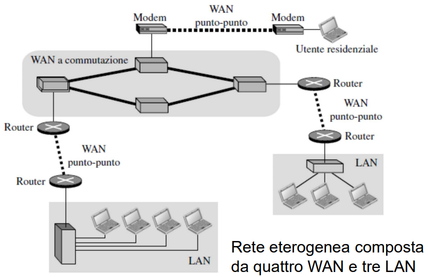
\includegraphics[width=\textwidth]{Immagini/Internetwork.png}
	\centering
	\caption{Una internetwork.}
\end{figure}\newline
\textit{Problema: come mandare informazioni da un host a un altro?}


\subsubsection{Reti a commutazione di circuito}
Nelle \textbf{reti a commutazione di circuito} le \textbf{risorse} sono \textbf{riservate end to end} per ogni connessione. Risulta quindi necessario il \textbf{setup della comunicazione} per instaurare la connessione ed elargire le risorse.\newline
La risorsa non è tutto il link, bensì si considerano come risorse la capacità o la larghezza di banda porzionate per ogni connessione. Le risorse assegnate rimangono inattive se non utilizzate (\textit{e.g. telefonata}). I dispositivi mantengono lo stato della connessione. \textbf{Le performance sono garantite}. La capacità delle linee (\textit{link}) cambia a seconda della loro funzione all'interno della rete. Il \textbf{punto debole} delle reti a commutazione di circuito è la \textbf{poca flessibilità nel dispiegamento delle risorse}.

\newpage

\subsubsection{Reti a commutazione di pacchetto}
Nelle \textbf{reti a commutazione di pacchetto} gli utenti inviano pacchetti che condividono le risorse del canale di comunicazione. \textbf{Non c'è} quindi \textbf{un canale dedicato} ai pacchetti di un singolo utente. La principale differenza rispetto alla commutazione di circuito risiede nell'implementazione della logica dei dispositivi di interconnessione, ovvero:
\begin{itemize}
	\item \textbf{Commutazione di Circuito}: avviene il \textbf{setup} della connessione dove  si prealloca l’utilizzo del collegamento trasmissivo con collegamenti
	      garantiti.
	\item \textbf{Commutazione di Pacchetto}: non viene instaurata una connessione bensì le informazioni necessarie si trovano all'interno dei pacchetti stessi, non ci sono informazioni di connessione memorizzate nei dispositivi coinvolti.
\end{itemize}
Nelle reti a commutazione di pacchetto quindi le risorse vengono usate a seconda della necessità. Possono quindi verificarsi situazioni di contesa delle risorse e sussiste il pericolo di congestione o di perdita dei pacchetti nel caso in cui la dimensione della coda del router non fosse sufficiente a contenere il flusso dei pacchetti entranti: il commutatore (\textit{router}) deve infatti ricevere l’intero
pacchetto prima di poter cominciare a trasmetterlo sul collegamento in uscita (\textit{\textbf{store and forward}}). \textbf{Non sono} quindi \textbf{garantite le prestazioni}.
\begin{figure}[!h]
	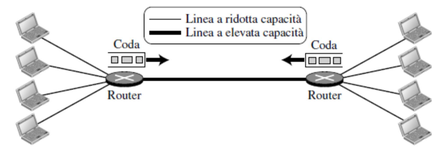
\includegraphics[width=\textwidth]{Immagini/Packet_Switch.png}
	\centering
	\caption{Rete a commutazione di pacchetto. Da notare le diverse capacità dei link.}
\end{figure}
\newpage
\subsubsection{Packet Switch e Circuit Switch a confronto}
Vi sono 35 utenti su una rete con 100 Kbit/s di connessione e un link da 1 Mbit/s.
Ogni utente è attivo solo il 10\% del tempo.\newline
Con una \textbf{rete a commutazione di circuito} si riescono a gestire \textbf{solo} 10 utenti.\newline
Con una \textbf{rete a commutazione di pacchetto} si hanno i seguenti casi:
\begin{enumerate}
	\item 10 o meno utenti attivi: nessun problema.
	\item Più di 10 utenti attivi: ritardo.
\end{enumerate}
Tuttavia che gli utenti siano tutti e 35 attivi contemporaneamente è poco probabile (infatti $P(35) = 0.0004$).
Se ne deduce che la rete a commutazione di pacchetto riesce a gestire tutti gli utenti contemporaneamente nella maggior parte dei casi.

Nonostante il risultato ottenuto non si deve pensare che la rete a  commutazione di circuito sia obsoleta. Nel corso degli anni infatti le due tecnologie sono state \textbf{integrate} in vari modi.\newline
La commutazione di circuito infatti è usata nella telefonia fissa (\textit{PSTN: public switch telephone network}) per i servizi voce, la commutazione di pacchetto invece per i dati.\newline
Nelle reti ottiche di prima e seconda generazione si usano entrambe le tecnologie.

\subsubsection{Circuiti virtuali}
I circuiti virtuali funzionano nel seguente modo: viene stabilito un path tra host sorgente e host destinazione e tutti i pacchetti di un certo flusso seguono lo \textbf{stesso} path.
\subsubsection{Datagram Network}
Con \textbf{datagram} si indica un'entità informativa autocontenuta che contiene le informazioni sufficienti per essere indirizzata alla destinazione senza comunicazioni aggiuntive tra sorgente e destinazione: \textbf{non è quindi detto} che pacchetti di uno stesso flusso seguano lo stesso path sulla rete.
\newpage

\subsection{Internet}
\textit{Come interconnettere reti già esistenti?}\newline
\theoremstyle{definition}
\begin{definition}
	Una internet (con i minuscola) è una rete costituita da
	due o più reti interconnesse.
\end{definition}
La internet più famosa è chiamata \textbf{Internet} (con i maiuscola) ed è composta da migliaia di reti interconnesse. Ogni rete connessa ad Internet deve usare il protocollo IP e rispettare certe convenzioni su come vengono assegnati nomi e indirizzi.
Si possono facilmente aggiungere nuove reti. \newline Tuttavia è impensabile avere un link fisico tra ogni host, si hanno invece numerosi
dispositivi di interconnessione che permettono la comunicazione da un host all'altro e da un router all'altro.\newline
Uno scorcio delle \textbf{componenti di Internet}:
\begin{itemize}
	\item Miliardi di dispositivi interconnessi (e.g. hosts, end systems).
	\item Link di comunicazione (e.g. fibre ottiche, doppini telefonici,
	      cavi coassiali, onde radio).
	\item Routers: instradano pacchetti \textit{(sequenze)} di dati attraverso la rete.
\end{itemize}

\begin{figure}[!h]
	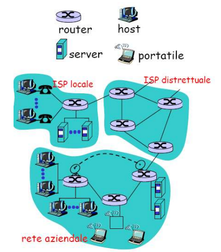
\includegraphics{Immagini/Internet.png}
	\centering
	\caption{Una porzione di Internet}
\end{figure}

\newpage

Uno scorcio delle \textbf{entità software} di Internet:

\begin{itemize}
	\item Applicazioni e processi che elaborano le informazioni.
	\item \textbf{Protocolli} che regolamentano la trasmissione e la ricezione di informazioni e.g. TCP, IP, HTTP, FTP, PPP.
	\item Interfacce: verranno definite in seguito, sono le \textit{“membrane”} che separano gli \textit{"strati"}.
\end{itemize}

\subsubsection{Servizi}
L’\textbf{infrastruttura di comunicazione} consente il funzionamento delle applicazioni distribuite per scambio di informazioni \textit{(e.g. WWW, email, giochi, e-commerce, database, controllo remoto, ecc).}\newline
Lo \textbf{stack protocollare} offre il servizio di connessione. Vi sono due approcci:
\begin{enumerate}
	\item \textbf{Connection-less}: I dati vengono trasferiti \textbf{senza} stabilire una
	      connessione, non c'è nessuna garanzia di ordine e consegna. \textit{Ogni pacchetto ha una vita a sè.}
	\item \textbf{Connection-oriented}: Prevede l'\textbf{instaurazione della connessione}, il trasferimento dei dati e, in seguito, la chiusura della connessione. Garantisce integrità, completezza e ordine.
\end{enumerate}

\subsubsection{IETF/RFC/ICANN}

\theoremstyle{definition}
\begin{definition}
	L'IETF (Internet Engineering Task Force) è l’organismo che studia e sviluppa i protocolli in uso su Internet. Si basa su gruppi di lavoro a cui chiunque può accedere.
\end{definition}

\theoremstyle{definition}
\begin{definition}
	RFC/STD (Request For Comments \& STanDards) sono i documenti \textit{“ufficiali” } che descrivono i protocolli usati su Internet. Sono pubblicamente accessibili in rete.
\end{definition}

\theoremstyle{definition}
\begin{definition}
	ICANN (Internet Corporation for Assigned Names and Numbers) È un ente internazionale che coordina il sistema dei nomi di dominio (DNS), assegna i gruppi di indirizzi di rete, identificativi di protocollo e ha funzioni di controllo (blando) dello sviluppo di Internet.
\end{definition}

\subsubsection{Rete di accesso}
Internet è una internetwork che consente a qualsiasi utente
di farne parte. L’utente, tuttavia, deve essere fisicamente collegato a un
ISP (\textit{internet service provider}).
\theoremstyle{definition}
\begin{definition}
	Il collegamento che connette l'utente al primo router di internet è detto \textbf{rete di accesso}, suddetto collegamento può essere effettuato tramite rete telefonica, rete wireless o tramite accesso diretto.
\end{definition}

\newpage

\begin{figure}[!h]
	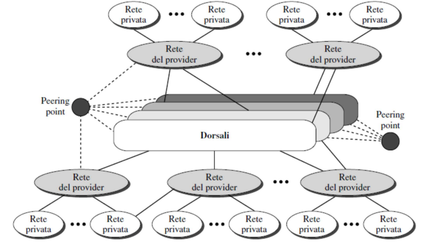
\includegraphics[width=\textwidth]{Immagini/Internet_Concept.png}
	\centering
	\caption{Un modello concettuale di Internet}
\end{figure}

\section{Metriche di riferimento}
\textit{Come misurare le prestazioni di una rete?}\newline

\theoremstyle{definition}
\begin{definition}
	La \textbf{larghezza di banda} o \textbf{bandwidth} è la larghezza dell'intervallo di frequenze utilizzato dal sistema trasmissivo.
\end{definition}

\theoremstyle{definition}
\begin{definition}
	Il \textbf{bit rate} o \textbf{trasmission rate} è la quantità di dati che possono essere trasmessi o ricevuti nell'unità di tempo. [e.g. bps = bit/s]\newline
	Il bitrate dipende dalla tecnica trasmissiva ed è proporzionale alla larghezza di banda.
\end{definition}

\theoremstyle{definition}
\begin{definition}
	Il \textbf{throughput} è la quantità di traffico che arriva realmente a destinazione nell'unità di tempo, al netto di perdite sulla rete,
	del funzionamento dei protocolli etc.
\end{definition}

\theoremstyle{definition}
\begin{definition}
	La \textbf{latenza} o \textbf{latency} è il tempo che passa dal momento in cui il primo bit parte dalla sorgente al momento in cui l'intero messaggio arriva a destinazione. \newline

	\fbox{\centering{$L = r_{propagazione} + r_{trasmissione} + r_{accomodamento} + r_{elaborazione}$}}
\end{definition}
\newpage

\subsection{Ritardi}
Il ritardo introdotto da un nodo è la somma di questi 4 ritardi:
\begin{figure}[!h]
	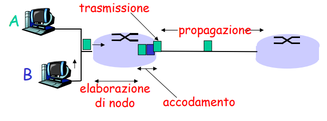
\includegraphics{Immagini/Ritardi.png}
	\centering
	\caption{Una visione di contesto}
\end{figure}

\subsubsection{Ritardo di elaborazione del nodo}
Il ritardo di elaborazione \textbf{è causato dall'elaborazione del percorso} (ovvero dove inoltrare il pacchetto scegliendo il percorso \textit{"migliore"}) \textbf{e dal controllo di errori sui bit}, è \textbf{tipicamente piccolo e trascurabile}.

\subsubsection{Ritardo di accodamento}
Il ritardo di accodamento \textbf{è il tempo che un pacchetto passa nella coda del router}, dipende dall'intensità e dal tipo di traffico. I pacchetti si accodano nei buffer dei router se il tasso di arrivo dei pacchetti eccede la capacità del collegamento di inoltrarli. Se non ci sono spazi liberi i pacchetti in arrivo vengono scartati.

\subsubsection{Rtardo di trasmissione}
Il ritardo di trasmissione \textbf{è il tempo impiegato a trasmettere un pacchetto intero} sul link.\newline
$R$ = rate di trasmissione del collegamento.\newline
$L$ = lunghezza del pacchetto.\newline
\centerline{$r_{trasmissione} = \frac{L}{R}$}

\subsubsection{Ritardo di propagazione}
Il ritardo di propagazione \textbf{è il tempo impiegato da un bit per essere propagato da un nodo (router) all'altro}.\newline
$d$ = lunghezza del collegamento fisico\newline
$s$ = velocità di propagazione del collegamento fisico \newline
\centerline{$r_{propagazione} = \frac{d}{s}$}

\subsection{Esempio}
Si consideri l'invio di un file di 1 MBit su un datalink di lunghezza 4800km:\newline
$d = 4800\times10^3 m$ \newline
$s = 3\times10^3 m/s$ \newline
Si calcoli il ritardo di propagazione. \newline
Soluzione:\newline
$r_{propagazione} = \frac{d}{s} = \frac{4800\times10^3 m }{3\times10^3 m/s}  = 0.016$ secondi.\newline
Sia il trasmission rate pari a 64 kbps, si calcoli il ritardo di trasmissione. \newline
$r_{trasmissione} = \frac{L}{R} = \frac{10^6 bit}{64\times10^3 bps}= 15.625$ secondi.\newline
Se il trasmission rate fosse invece di 1 Gbps? \newline
$r_{trasmissione} = \frac{L}{R} = \frac{10^6 bit}{10^9 bps} = 0.001$ secondi.

\subsection{Volume di un link}
\begin{figure}[!h]
	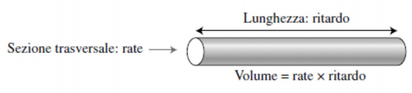
\includegraphics[width=\textwidth]{Immagini/Link_Volume.png}
	\centering
\end{figure}
\theoremstyle{definition}
\begin{definition}
	Il volume di un link è il numero massimo di bit che il link può contenere.
\end{definition}
\centerline{\fbox{$Volume = bit rate\times ritardo$}}

\subsection{Esempio}
\begin{figure}[!h]
	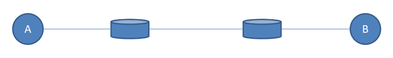
\includegraphics[width=\textwidth]{Immagini/Esempio_ritardi.png}
	\centering
\end{figure}
Si calcoli il ritardo end-to-end di un pacchetto su un percorso con due router. Sia trascurabile il ritardo di congestione e si suppongano uguali su tutti link il propagation delay, il transmission delay e il processing delay.\newline\newline
\textbf{Soluzione}:\newline Essendoci due router intermedi bisongna attraversare tre link, quindi:\newline
\centerline{$r_{totale} = 3\times r_{propagation} + 3\times r_{trasmission} + 3\times r_{processing}$}
\newpage
\begin{figure}[!h]
	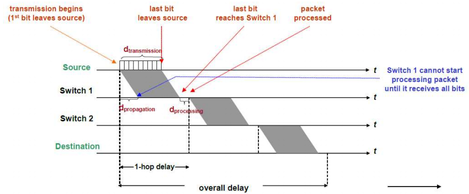
\includegraphics[width=\textwidth]{Immagini/Soluzione_ritardi.png}
	\centering
	\caption{Quello che succede in dettaglio.}
\end{figure}

\section{Modelli Stratificati e Protocolli}
\textit{Cos'è un protocollo? Cos'è uno strato?}
\subsection{Principi alla base della stratificazione di un sistema}
La stratificazione di un sistema è guidata dai seguenti principi:
\begin{itemize}
	\item Information hiding.
	\item Separation of concerns.
\end{itemize}
\begin{figure}[!h]
	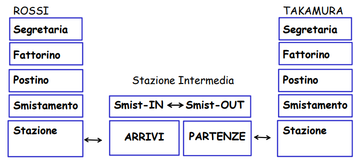
\includegraphics[width=\textwidth]{Immagini/Postale.png}
	\centering
	\caption{Esempio di stratificazione. Si nota come i vari strati del modello interagiscono tra di loro, dal basso verso l'alto e viceversa, per consentire al sig. Rossi e al sig. Takamura di scambiarsi lettere.}
\end{figure}
\newpage
Vantaggi della stratificazione:
\begin{itemize}
	\item \textbf{Facilità di progettazione.}
	\item \textbf{Facilità di manutenzione.}
	\item \textbf{Possibilità di riciclo.}
\end{itemize}

\textbf{\underline{N.B.}}:
\begin{enumerate}
	\item Gli strati comunicano \textit{(di solito)} \textbf{solo} con gli altri strati a loro adiacenti.
	\item Uno strato \textbf{fornisce} servizi allo strato superiore e \textbf{riceve} servizi da quello inferiore.
	\item La comunicazione tra strati adiacenti avviene attraverso un'\textbf{interfaccia}.
	\item Tra due entità diverse comunicano fra di loro solo gli strati dello \textbf{stesso livello} e secondo un \textbf{protocollo assegnato}, queste due entità sono dette \textbf{peer}.
\end{enumerate}


\subsection{OSI: Open Systems Interconnection}
Le \textbf{prime} reti di calcolatori nacquero come \textbf{sistemi chiusi} in cui tutti i componenti dovevano essere dello stesso costruttore. Erano quindi tecnologie chiuse e \textbf{non interoperabili} l'una con l'altra a causa di drastiche differenze \textit{(e.g. differenza di linguaggio, \textbf{modelli di stratificazione diversi} e impossibilità per i programmi applicativi di riuscire ad operare in ambiente distribuito)}. Alla fine degli anni ‘60 esistevano: ARPANET, SNA (IBM), DNA (Digital).\newline
I \textbf{Sistemi Aperti} nascono dall'obbiettivo di alcune aziende di realizzare una rete di calcolatori in cui qualsiasi terminale potesse comunicare con un qualsiasi fornitore di servizi mediante qualsiasi rete.\newline\newline
Per realizzare un sistema aperto è necessario stabilire delle regole comuni: \textbf{gli standards}.
\theoremstyle{definition}
\begin{definition}
	Un sistema che implementa \textbf{protocolli aperti} è un \textbf{sistema aperto} (open system).
\end{definition}
\begin{definition}
	Un set di protocolli è \textbf{aperto} se:
	\begin{enumerate}
		\item I dettagli (\textbf{specifiche}) dei protocolli sono disponibili pubblicamente.
		\item I cambiamenti al set sono gestiti da un’organizzazione la cui
		      partecipazione è aperta al pubblico
	\end{enumerate}
\end{definition}

\subsubsection{Modello ISO/OSI}
L’International Organization for Standards (ISO) ha specificato
uno standard per l’interconnessione di sistemi aperti: l' \textbf{Open System Interconnection Reference Model} (OSI-RM) poi diventato standard internazionale nel 1983 (ISO 7498). \textbf{Si basa sul concetto di architettura a strati i cui criteri sono:}.
\begin{itemize}
	\item \textbf{Divisione delle funzionalità}: il protocollo di telecomunicazione è diviso in strati o layers, ognuno dei quali svolge un compito piccolo e indipendente dagli altri.\newline
	      Si cerca quindi di mantenere un minor numero di strati possibile e di far svolgere a ognuno di essi il minor numero di compiti possibile.
	\item \textbf{Comunicazione mediante interfacce}: i livelli comunicano mediante \textbf{chiamate standard}. Ogni livello è tenuto a rispondere alle \textbf{sole} chiamate che gli competono e che verranno
	      invocate dai due livelli ad esso adiacenti.
	\item \textbf{Information hiding}: le modalità con cui le funzioni competenti ad un livello
	      vengono svolte non è visibile dall'esterno che ne è così
	      svincolato.
\end{itemize}

\subsection{Protocollo}
\begin{figure}[!h]
	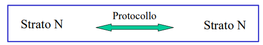
\includegraphics[width=\textwidth]{Immagini/Protocollo.png}
	\centering
\end{figure}
I protocolli definiscono il \textbf{formato} e l’\textbf{ordine} dei
messaggi inviati e ricevuti tra entità della rete al livello n-esimo e
le \textbf{azioni} che vengono fatte per la loro \textbf{trasmissione} e
\textbf{ricezione}.
\theoremstyle{definition}
\begin{definition}
	Un \textbf{protocollo} è un insieme di regole che permettono a due entità uno scambio \textbf{efficace} ed \textbf{efficiente} delle informazioni. \textbf{Definisce} il \textbf{formato} e il
	\textbf{significato} dei frame (campi del messaggio), dei pacchetti o dei messaggi
	che vengono scambiati tra gli \textbf{strati paritari} di due
	entità diverse.
\end{definition}
Un protocollo specifica quindi:
\begin{itemize}
	\item La \textbf{sintassi} di un messaggio (e.g. i campi).
	\item La \textbf{semantica}.
	\item  \textbf{Le azioni da compiere }(e.g. per l'invio, alla ricezione, alla trasmissione etc...).
\end{itemize}
\theoremstyle{definition}
\begin{definition}
	Uno \textbf{strato} o livello è un modulo interamente definito attraverso i
	servizi, protocolli e le interfacce che lo caratterizzano.
\end{definition}
\theoremstyle{definition}
\begin{definition}
	Un' \textbf{interfaccia} è il set di regole governanti sintassi e semantica della comunicazione tra due \textbf{strati successivi} della \textbf{stessa entità}.
\end{definition}
\theoremstyle{definition}
\begin{definition}
	Un \textbf{servizio} è insieme di \textbf{primitive} (operazioni) che uno strato
	fornisce ad uno strato soprastante. (\textit{vedi sez. 3.4.1}).
\end{definition}
\begin{figure}[!h]
	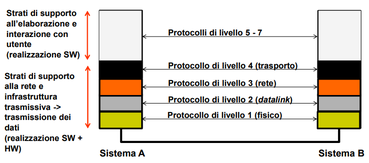
\includegraphics[width=\textwidth]{Immagini/Protocol_stack.png}
	\centering
	\caption{Esempio di stack protocollare.}
\end{figure}
\begin{figure}[!h]
	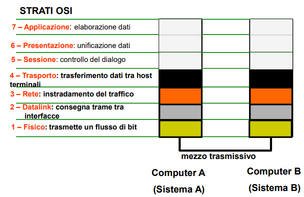
\includegraphics[width=\textwidth]{Immagini/Osi_strati.png}
	\centering
	\caption{Gli strati di OSI.}
\end{figure}
\begin{figure}[!h]
	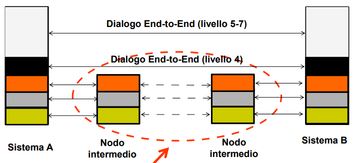
\includegraphics[width=\textwidth]{Immagini/End_sys.png}
	\centering
	\caption{Esempio di collegamento tra end systems.}
\end{figure}
\newpage
\subsection{Incapsulamento dell'informazione}
All'interno della rete l'informazione ha origine \textbf{al livello
	applicativo} (\textit{livello 7 in figura}), discende quindi i vari livelli fino alla
\textbf{trasmissione}, che avviene mediante il \textbf{canale fisico}.
Da ogni livello attraversato viene aggiunta all'informazione una sezione informativa (o più di una) chiamata \textbf{header} che contiene informazioni pertinenti esclusivamente al livello stesso.
Per i dati ricevuti invece si segue il cammino inverso. Si tratta infatti di un \textbf{processo di incapsulamento \underline{reversibile}}.
\begin{figure}[!h]
	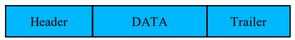
\includegraphics[width=\textwidth]{Immagini/Incapsulamento.png}
	\centering
\end{figure}
\begin{itemize}
	\item \textbf{Header}: è qualificazione del pacchetto dati per questo livello.
	\item \textbf{DATA}: è il payload proveniente dal livello superiore.
	\item \textbf{Trailer}: è usato per rilevare e correggere gli errori.
\end{itemize}

\begin{figure}[!h]
	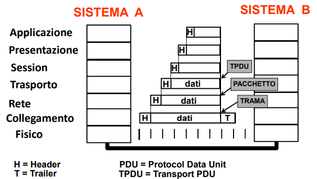
\includegraphics[width=\textwidth]{Immagini/Incaps_2.png}
	\centering
	\caption{Il processo di incapsulamento. Da notare in particolare il payload.}
\end{figure}
\newpage

\subsection{Stack protocollare TCP/IP}
\textbf{TCP/IP} è una \textbf{famiglia di protocolli} attualmente
in uso su Internet.\newline Si tratta di una \textbf{gerarchia di
	protocolli} costituita da \textbf{moduli interagenti}, ciascuno dei
quali fornisce funzionalità specifiche.
Il termine \textbf{gerarchia} significa che ciascun protocollo di
\textbf{livello superiore} è supportato dai servizi \textbf{forniti} dai
protocolli di \textbf{livello inferiore}.
Definita in origine in termini di quattro livelli software
soprastanti a un livello hardware, \textbf{la pila TCP/IP} è \textbf{oggi}
intesa come \textbf{composta} \textbf{di cinque livelli}.
\begin{figure}[!h]
	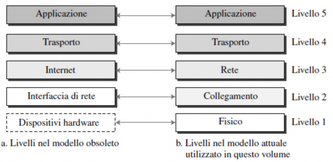
\includegraphics[width=\textwidth]{Immagini/TCP_IP.png}
	\centering
	\caption{Livelli dello stack protocollare TCP/IP, si notino le differenze tra il modello originario e il modello attuale.}
\end{figure}

\begin{figure}[!h]
	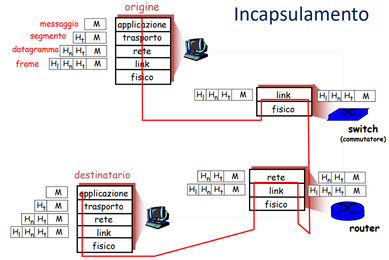
\includegraphics[width=\textwidth]{Immagini/Incapsulamento_m.png}
	\centering
	\caption{Esemplificazione del processo di incapsulamento/decapsulamento dell'informazione.}
\end{figure}

\begin{figure}[!h]
	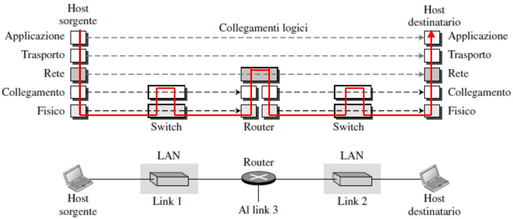
\includegraphics[width=\textwidth]{Immagini/Logfis.png}
	\centering
	\caption{I vari collegamenti logici di comunicazione, in \textbf{rosso} invece, \textbf{il collegamento fisico}. La modularità del sistema fa in modo che gli strati paritari dei due host abbiano l'\textbf{illusione} di comunicare direttamente tra di loro. Si ricorda che queste entità situate a livelli corrispondenti su macchine (host) diverse sono dette \textbf{peer}.}
\end{figure}

\end{document}









